\documentclass{article}
\usepackage[en]{homework}
\usepackage{tensor}

\config{Physics\,-\,0}{2026 Spring}{1}

% TikZ Settings
\usepackage{pgfplots}
\pgfplotsset{compat=1.15}
\usepackage{mathrsfs}
\usetikzlibrary{arrows}
\definecolor{qqffff}{rgb}{0.,1.,1.}
\definecolor{qqqqff}{rgb}{0.,0.,1.}
\definecolor{ffqqqq}{rgb}{1.,0.,0.}
\definecolor{qqwwtt}{rgb}{0.,0.4,0.2}
\definecolor{yqyqyq}{rgb}{0.5019607843137255,0.5019607843137255,0.5019607843137255}


\begin{document}

Notice: Take $ g=10 \mathrm{m/s^2} $ for numerical calculation.

\begin{problem}
(45pts)A ball is thrown straight up from the edge of the roof of a building. A second ball is dropped from the roof 1s later. Ignore air resistance. Answer the following questions:

\begin{enumerate}[label=(\alph*)]
    \item (5pts) As these balls fall, does the distance between them increase, decrease, or remain the same?
    \item (10pts) If the height of the building is \(20\,\text{m}\), what must the initial speed of the first ball be if both are to hit the ground at the same time? On the same graph, sketch the positions of both balls as a function of time, measured from the time when the first ball is thrown. Consider the same situation, but now let the initial speed \(v_{0}\) of the first ball be given and treat the height \(h\) of the building as an unknown.
    \item (10pts) What must the height of the building be for both balls to reach the ground at the same time if (i) \(v_{0} = 6.0\,\text{m}/\text{s}\) and (ii) \(v_{0} = 9.5\,\text{m}/\text{s}\)?
    \item (10pts) If \(v_{0} > v_{\mathrm{max}}\) for some value \(v_{\mathrm{max}}\), no value of \(h\) exists that allows both balls to hit the ground at the same time. Solve for \(v_{\mathrm{max}}\). The value \(v_{\mathrm{max}}\) has a simple physical interpretation. What is it?
    \item (10pts) If \(v_{0} < v_{\mathrm{min}}\), no value of \(h\) exists that allows both balls to hit the ground at the same time. Solve for \(v_{\mathrm{min}}\). The value \(v_{\mathrm{min}}\) also has a simple physical interpretation. What is it?
\end{enumerate}
\end{problem}

\begin{solution}
Suppose the first ball is thrown with an initial speed \(v_0\) , and the height of the building is \(h\). Choose the top of the building as the origin of the coordinate system, and let the positive direction be upward. Take $ t_0=1\mathrm{s}. $The position of the two balls as a function of time \(t\) is given by

\[ x_1(t)=v_0t-\frac{1}{2}gt^2,\quad, x_2(t)=
\begin{cases}
0, & t<t_0;\\
-\frac{1}{2}g(t-t_0)^2, & t\geq t_0.
\end{cases}\] 

(a) We only need to consider the situation when \(t\geq t_0\). The distance between the two balls is given by
\[ d(t)=\abs{x_1(t)-x_2(t)}=\abs{v_0t-\frac{1}{2}gt^2+\frac{1}{2}g(t-t_0)^2}=\abs{(v_0-gt_0)t+\frac{1}{2}gt_0^2}.\]
Then we need to discuss about different cases:
\begin{enumerate}[label=(\roman*)]
    \item If \(v_0>gt_0\), then \(d(t)\) is an increasing function of \(t\). So the distance between the two balls increases.
    \item If \(v_0=gt_0\), then \(d(t)\) is a constant. So the distance between the two balls remains the same.
    \item If \(v_0<gt_0\), then \(d(t)\) decreases when \(t<\dfrac{gt_0^2}{2(gt_0-v_0)}\) and increases when \(t>\dfrac{gt_0^2}{2(gt_0-v_0)}\). So the distance between the two balls first decreases and then increases.
\end{enumerate}

(b) Suppose the first ball hits the ground at time \(t_1\), and the second ball hits the ground at time \(t_2\). Then we have
\[ x_1(t_1) = 0 \quad \text{and} \quad x_2(t_2) = 0. \]
Solving these equations gives
\[ t_1 = \frac{v_0 + \sqrt{v_0^2 + 2gh}}{g} \quad \text{and} \quad t_2 = t_0 + \sqrt{\frac{2h}{g}}. \]
Set \(t_1 = t_2\) , we got the expressiong of $ v_0 $:
\[ v_0=\frac{g^2 t_0^2 \left(\sqrt{2h/g}+t_0\right)-4 g t_0h}{2 g t_0^2-4 h}. \]
Take $ h=20\,\mathrm{m} $, we got $ \boxed{v_0=8.33\,\mathrm{m/s}} $.
We can also solve the height of the building \(h\) as a function of \(v_0\):
\[ \boxed{h=\frac{g t_0^2 (g t_0-2 v_0)^2}{8 (v_0-g t_0)^2}}. \] \par 

(c) Take \(v_0 = 6.0\,\text{m}/\text{s}\) into the expression of \(h\), we got $ \boxed{h=0.3125\,\mathrm{m}} $. Take \(v_0 = 9.5\,\text{m}/\text{s}\) into the expression of \(h\), we got $ \boxed{h=405\,\mathrm{m}} $.\par 

(d) and (e)\ \ We only need to ditermine the range of $ v_0 $ where the equation
\[ x_1(t)=x_2(t),\quad t\ge t_0 \] 
has a solution. By solving this mathmatical problem, we got
\[ \frac{1}{2}gt_0\le v_0\le gt_0. \] \par 
Then $ \boxed{v_\mathrm{max}=gt_0=10\,\mathrm{m/s}} $. The physical interpretation of \(v_{\mathrm{max}}\) can be explained as follows: The velocity of the first ball at time \(t_0\) is given by \(v_0 - gt_0\). If \(v_0 > gt_0\), then the first ball is still moving upward at time \(t_0\) when the second ball is dropped. Choose the co-moving reference frame w.r.t the second ball, the first ball is moving upward with a constant nonzero velocity $ v_0-gt_0 $. So the first ball will always be above the second ball, and they can never hit the ground at the same time.\par 
Also, we have got $ \boxed{v_\mathrm{min}=gt_0/2=5\, \mathrm{m/s}} $. The physical interpretation of $ v_{\mathrm{min}} $ can be explained as follows: If $ v_0 < \frac{1}{2}gt_0 $, then the first ball meets the second ball before the departure of the second ball, then the first ball will always be below the second ball. So they can never hit the ground at the same time.
\end{solution}


\begin{problem}
(55pts) Consider a frame \(O'\) rotating with respect to a frame \(O\) around the \(z\) axis at angular speed \(\omega = \dot{\theta}(t)\), where \(\theta(t)\) is the angle of rotation (see figure below). The angular velocity vector \(\bo{\omega}\) is a vector that points along the axis of rotation (the \(z\)-axis) with magnitude \(\omega\), i.e.
\[
\bo{\omega} = \omega \hat{z}. \tag{1}
\]
Let \(\bo{e}_{i}\) with \(i = 1,2,3\) denote the unit vectors of frame \(O\) along the \(x, y,\) and \(z\) directions, respectively, i.e. \((\bo{e}_{1},\bo{e}_{2},\bo{e}_{3}) = (\hat{x},\hat{y},\hat{z})\). (The unit vectors satisfy \(\bo{e}_{i}\cdot \bo{e}_{i} = 1\) for all \(i\) and \(\bo{e}_{i}\cdot \bo{e}_{j} = 0\) for all \(i\neq j\).) Similarly, let \(\bo{e}_{i}'\) denote the unit vectors of the frame \(O'\). Since the \(z\)-axis does not rotate, we have \(\bo{e}_{3} = \bo{e}_{3}'\).

\begin{center}
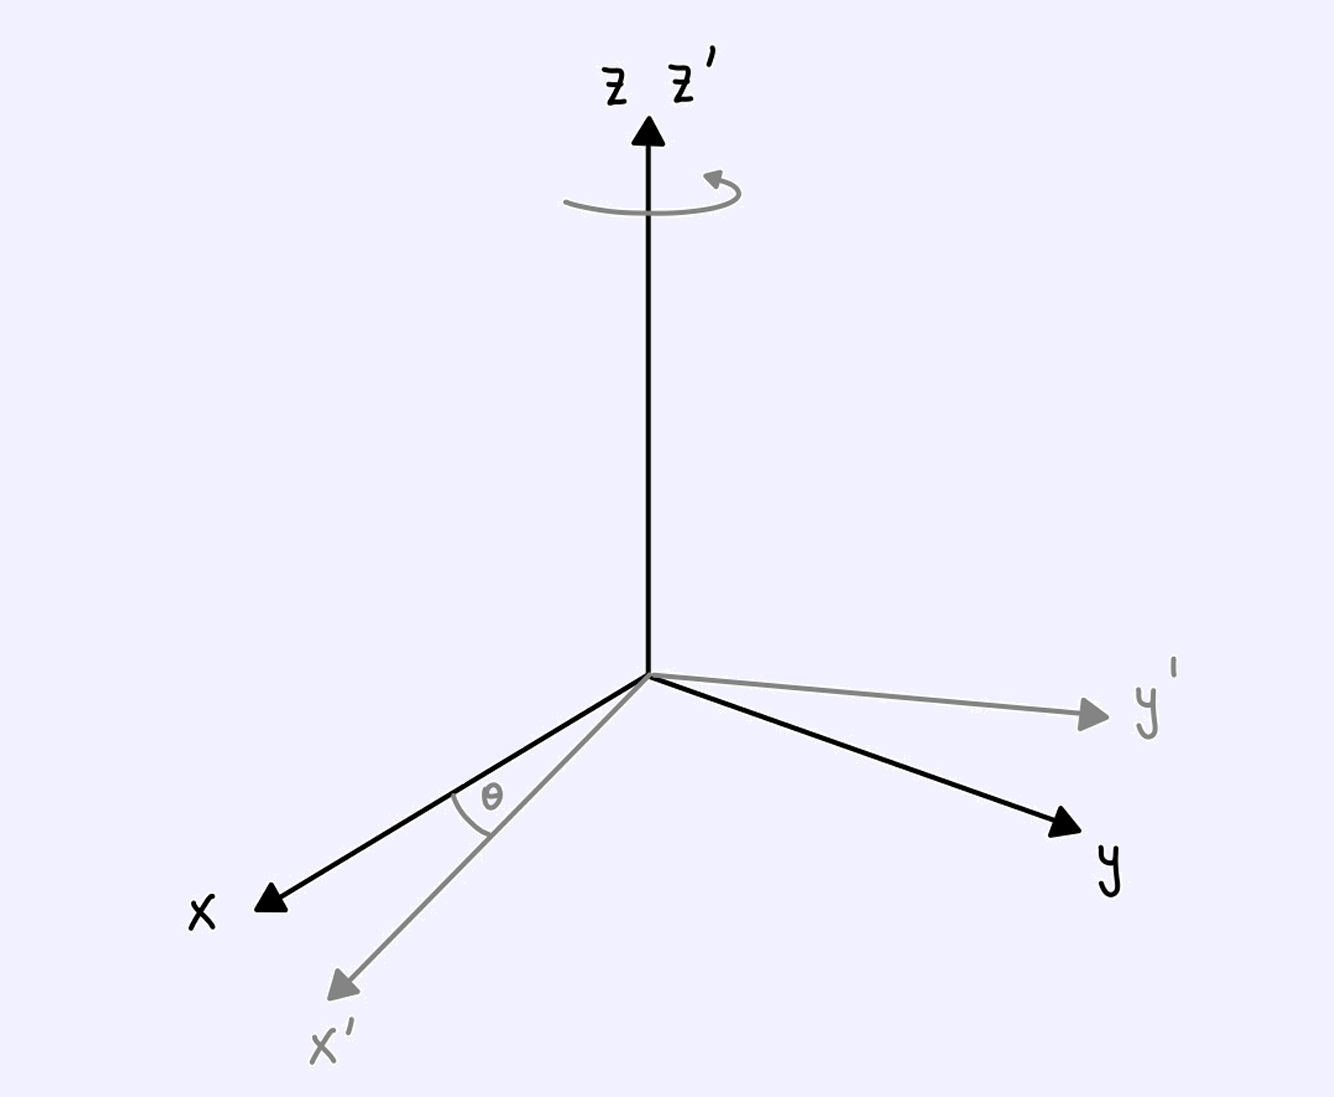
\includegraphics[width=0.5\textwidth]{Problem2.png}
\end{center}

\begin{enumerate}[label=(\alph*)]
    \item (10pts) Let \(\bo{r}\) denote the position of the particle in frame \(O\). Show that, from the point of view of \(O\), a particle at rest in \(O'\) moves with velocity
    \[
    \dot{\bo{r}} = \bo{\omega}\times \bo{r} \tag{2}
    \]
    where the cross product between the basis vectors is given by
    \[
    \bo{e}_{i}\times \bo{e}_{j} = \sum_{k = 1}^{3}\epsilon_{ijk}\bo{e}_{k} \tag{3}
    \]
    where \(\epsilon_{ijk}\) is the totally antisymmetric Levi-Civita symbol defined such that \(\epsilon_{ijk} = 1\) for any even permutation of \((i,j,k) = (1,2,3)\), e.g. \(\epsilon_{123} = \epsilon_{312} = 1\), while \(\epsilon_{ijk} = -1\) for any odd permutation, e.g. \(\epsilon_{132} = \epsilon_{213} = -1\).
    \item (5pts) Similarly, show that the unit vectors of the frame \(O'\) rotate with velocity
    \[
    \dot{\bo{e}}_i' = \bo{\omega}\times \bo{e}_i' \tag{4}
    \]
    \item (10pts) Denote by \(\dot{\bo{r}}_O = \sum_{i = 1}^{3}\dot{r}_i\bo{e}_i\) the velocity observed from frame \(O\), and by \(\dot{\bo{r}}_{O'} = \sum_{i = 1}^{3}\dot{r}_i'\bo{e}_i'\) the velocity observed from frame \(O'\). Show that
    \[
    \dot{\bo{r}}_O = \dot{\bo{r}}_{O'} + \bo{\omega}\times \bo{r} \tag{5}
    \]
    \item (15pts) Compute the accelerations \(\ddot{\bo{r}}_O\) and \(\ddot{\bo{r}}_{O'}\). Since \(O'\) is not an inertial frame, these accelerations are not equal, but are related by the addition of extra terms (three in total). These terms lead to fictitious forces that arise from working in a non-inertial frame.
    \item (15pts) Show in a diagram the directions where the fictitious forces point given some vector \(\bo{r}\).
\end{enumerate}
\end{problem}

\begin{solution}

The Einstein summation convention is used in the following calculations. For example, we will write \(\bo{r} = r^i \bo{e}_i\) instead of \(\bo{r} = \sum_{i=1}^{3} r^i \bo{e}_i\).
Note that we will not distinguish the upper and lower indices in the following calculations, especially when we are using the Levi-Civita symbol. For example. $ \epsilon_{ijk}=\epsilon\indices{_{ij}^k}. $

(a) Suppose the position of the particle is given by \(\bo{r} = r^i\bo{e}_i = r'^i \bo{e}'_i\). Since the particle is at rest in frame \(O'\), we have \(\dot{r}'^i = 0\) for all \(i\). Then, from the reference frame transformation rule, we have
\[ r^1=r'^1\cos(\omega t)-r'^2\sin(\omega t),\ r^2=r'^1\sin(\omega t)+r'^2\cos(\omega t),\ r^3=r'^3 \tag{6} \]
By taking the time derivative of the above equations, we got
\[ \dot{r}^1=-\omega r'^1\sin(\omega t)-\omega r'^2\cos(\omega t),\ \dot{r}^2=\omega r'^1\cos(\omega t)-\omega r'^2\sin(\omega t),\ \dot{r}^3=0. \]
Denote the components of $ \bo{\omega} $ as $ \omega^1=\omega^2=0,\omega^3=\omega $.
Then
\begin{align*}
\dot{\bo{r}}=&\dot{r}^i\bo{e}_i=\left\{-\omega r'^1\sin(\omega t)-\omega r'^2\cos(\omega t)\right\}\bo{e}_1 +\left\{\omega r'^1\cos(\omega t)-\omega r'^2\sin(\omega t)\right\}\bo{e}_2\\
=&\omega r'^1\left\{-\sin(\omega t)\bo{e}_1+\cos(\omega t)\bo{e}_2\right\}
+\omega r'^2\left\{-\cos(\omega t)\bo{e}_1-\sin(\omega t)\bo{e}_2\right\}\\
=&\omega r'^1\bo{e}_2'-\omega r'^2\bo{e}_1'=\epsilon\indices{_{ij}^k}\omega^i r'^j\bo{e}_k'=\omega^i r'^j(\bo{e}_i'\times\bo{e}_j')=(\omega^i\bo{e}_i')\times(r'^j\bo{e}_j')\\
=&\bo{\omega}\times \bo{r}.
\end{align*}

(b) This is a corally of (a), since the unit vectors of frame \(O'\) are also at rest in frame \(O'\).

(c) By Convention, we will denote the components of \(\dot{\bo{r}}_O\) as \(\dot{\bo{r}}_O=\dot{r}^i\bo{e}_i\) and the components of \(\dot{\bo{r}}_{O'}\) as \(\dot{\bo{r}}_{O'}=\dot{r}^{\prime i}\bo{e}_i'\). Then we only need to verify that
\[ \dot{r}^k\bo{e}_k=\dot{r}^{\prime k}\bo{e}_k'+\epsilon\indices{_{ij}^k}\omega^i r^j\bo{e}_k. \]

By taking the time derivative of the equation (6), we got
\[ \dot{r}^1=\dot{r}'^1\cos(\omega t)-\dot{r}'^2\sin(\omega t)-\omega r'^1\sin(\omega t)-\omega r'^2\cos(\omega t), \]
\[ \dot{r}^2=\dot{r}'^1\sin(\omega t)+\dot{r}'^2\cos(\omega t)+\omega r'^1\cos(\omega t)-\omega r'^2\sin(\omega t), \]
\[ \dot{r}^3=\dot{r}'^3. \]
Then we can verify that
\[ \left\{\dot{r}'^1\cos(\omega t)-\dot{r}'^2\sin(\omega t)\right\}\bo{e}_1 +\left\{\dot{r}'^1\sin(\omega t)+\dot{r}'^2\cos(\omega t)\right\}\bo{e}_2 +\dot{r}'^3\bo{e}_3=\dot{r}^{\prime k}\bo{e}_k' \]
by
\[ \left(\begin{matrix}
\bo{e}_1'\\ \bo{e}_2' \\ \bo{e}_3'
\end{matrix}\right)
=\left(\begin{matrix}
\cos(\omega t) & \sin(\omega t) & 0\\
-\sin(\omega t) & \cos(\omega t) & 0\\
0 & 0 & 1
\end{matrix}\right)\left(\begin{matrix}
\bo{e}_1\\ \bo{e}_2 \\ \bo{e}_3
\end{matrix}\right), \]
and \[ \epsilon\indices{_{ijk}}\omega^i r^j\bo{e}_k=\left\{-\omega r'^1\sin(\omega t)-\omega r'^2\cos(\omega t)\right\}\bo{e}_1 +\left\{\omega r'^1\cos(\omega t)-\omega r'^2\sin(\omega t)\right\}\bo{e}_2 \]
by $ (\omega^1,\omega^2,\omega^3) = (0,0,\omega) $ and 
\[ \left(\begin{matrix}
r'_1\\r'_2\\r'_3
\end{matrix}\right)
=\left(\begin{matrix}
\cos(\omega t) & \sin(\omega t) & 0\\
-\sin(\omega t) & \cos(\omega t) & 0\\
0 & 0 & 1
\end{matrix}\right)\left(\begin{matrix}
r_1\\r_2\\r_3
\end{matrix}\right).\] 
Then the equation (5) is verified.

(d) By taking the two-order time derivative of the equation (6), we got
\begin{align*}
\ddot{r}^1=&-\omega^2\left\{\cos(\omega t)r'^1-\sin(\omega t)r'^2\right\}\\
&+2\omega\left\{-\dot{r}'^1\sin(\omega t)-\dot{r}'^2\cos(\omega t)\right\}
+\left\{\ddot{r}'^1\cos(\omega t)-\ddot{r}'^2\sin(\omega t)\right\},\\
\ddot{r}^2=&-\omega^2\left\{\sin(\omega t)r'^1+\cos(\omega t)r'^2\right\}\\
&+2\omega\left\{\dot{r}'^1\cos(\omega t)-\dot{r}'^2\sin(\omega t)\right\}
+\left\{\ddot{r}'^1\sin(\omega t)+\ddot{r}'^2\cos(\omega t)\right\},\\
\ddot{r}^3=&\ddot{r}'^3.
\end{align*}

Denote $ \bo{r}_{\parallel} = r^1\bo{e}_1+r^2\bo{e}_2 = r'^1\bo{e}_1'+r'^2\bo{e}_2' $. Then we can verify (by the reference frame transformation rule) that
\begin{align*}
\left\{\cos(\omega t)r'^1-\sin(\omega t)r'^2\right\}\bo{e}_1
+\left\{\cos(\omega t)r'^1-\sin(\omega t)r'^2\right\}\bo{e}_2
&=-\omega^2 r_{\parallel}^i \bo{e}_i=-\omega^2\bo{r}_{\parallel}, \\
2\omega\left\{-\dot{r}'^1\sin(\omega t)-\dot{r}'^2\cos(\omega t)\right\}\bo{e}_1
+2\omega\left\{\dot{r}'^1\cos(\omega t)-\dot{r}'^2\sin(\omega t)\right\}\bo{e}_2
&=2\dot{\bo{r}}\times\bo{\omega}, \\
\left\{\ddot{r}'^1\cos(\omega t)-\ddot{r}'^2\sin(\omega t)\right\}\bo{e}_1
+\left\{\ddot{r}'^1\sin(\omega t)+\ddot{r}'^2\cos(\omega t)\right\}\bo{e}_2
+\ddot{r}^3\bo{e}_3
&=\ddot{r}^i\bo{e}_i=\ddot{\bo{r}}.
\end{align*}
Asemble the above equations together, we got
\[ \ddot{\bo{r}} = \ddot{\bo{r}}' + 2\dot{\bo{r}}'\times \bo{\omega} -\omega^2\bo{r}_{\parallel}. \]

(e) We will give a 2D diagram , looking from the positive $ z $ axis, since the problem is symmetric about the \(z\)-axis. 

\begin{figure}[htbp]
\centering
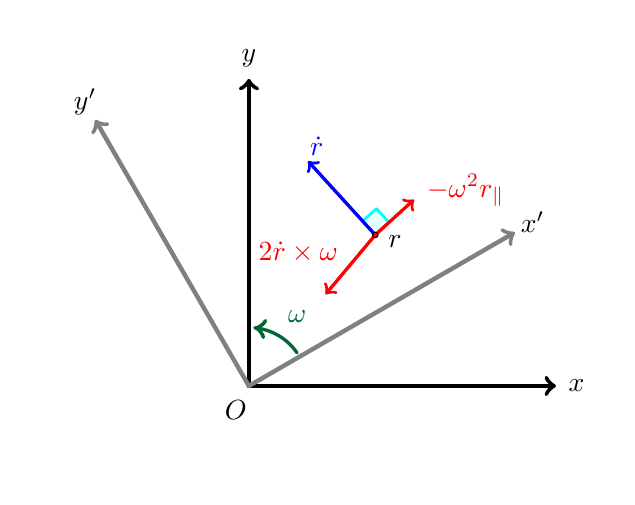
\begin{tikzpicture}[line cap=round,line join=round,x=1.3cm,y=1.3cm]
\clip(-2.1612470806998356,-0.889799922832837) rectangle (3.5,3.5);
\draw[line width=1.pt,color=qqffff,fill=qqffff,fill opacity=0.10000000149011612] (1.3690915568150608,1.597792480125121) -- (1.2463349403343753,1.732604256376454) -- (1.1115231640830425,1.6098476398957686) -- (1.2342797805637278,1.4750358636444356) -- cycle; 
\draw [->,line width=1.6pt] (0.,0.)-- (3.,0.);
\draw [->,line width=1.6pt] (0.,0.)-- (0.,3.);
\draw [->,line width=1.6pt,color=yqyqyq] (0.,0.)-- (2.598076211353316,1.5);
\draw [->,line width=1.6pt,color=yqyqyq] (0.,0.)-- (-1.5,2.598076211353316);
\draw [shift={(0.,0.)},line width=1.2pt,color=qqwwtt]  plot[domain=0.6004324223801785:1.4694031096361908,variable=\t]({1.*0.570722474146846*cos(\t r)+0.*0.570722474146846*sin(\t r)},{0.*0.570722474146846*cos(\t r)+1.*0.570722474146846*sin(\t r)});
\draw [->,line width=1.6pt,color=qqwwtt] (0.08130275068985032,0.5649017659970281)-- (0.05776828695148349,0.5677913063080379);
\draw [->,line width=1.2pt,color=qqqqff] (1.2342797805637278,1.4750358636444356)-- (0.5780728022911256,2.1956848263288093);
\draw [->,line width=1.2pt,color=ffqqqq] (1.2342797805637278,1.4750358636444356)-- (1.6125122851321652,1.8194460019492311);
\draw [->,line width=1.2pt,color=ffqqqq] (1.2342797805637278,1.4750358636444356)-- (0.7492052007204015,0.8953436309122638);
\draw (-0.3305095844581348,-0.047488774327265684) node[anchor=north west] {$O$};
\draw (3.2,0.) node {$x$};
\draw (0,3.2) node {$y$};
\draw (2.77128,1.6) node {$x'$};
\draw (-1.6,2.771283) node {$y'$};
\draw [color=qqwwtt](0.28833125934187687,0.8292024210560841) node[anchor=north west] {$\boldsymbol{\omega}$};
\draw (1.268162595358562,1.5597784172088756) node[anchor=north west] {$\boldsymbol{r}$};
\draw [color=qqqqff](0.503206552327992,2.531014741506116) node[anchor=north west] {$\dot{\boldsymbol{r}}$};
\draw [color=ffqqqq](1.6463431110141247,2.161429237569998) node[anchor=north west] {$-\omega^2\boldsymbol{r}_{\parallel}$};
\draw [color=ffqqqq](0,1.5) node[anchor=north west] {$2\dot{\boldsymbol{r}}\times\boldsymbol{\omega}$};
\begin{scriptsize}
\draw [fill=ffqqqq] (1.2342797805637278,1.4750358636444356) circle (1.0pt);
\end{scriptsize}
\end{tikzpicture}
\end{figure}


\end{solution}

\end{document}